\documentclass[10pt, aspectratio=169, handout]{beamer}
\usefonttheme{professionalfonts}
%\usetheme{CambridgeUS}
%
% Choose how your presentation looks.
%
% For more themes, color themes and font themes, see:
% http://deic.uab.es/~iblanes/beamer_gallery/index_by_theme.html
%
\mode<presentation>
{
  \usetheme{Berkeley}      % or try Darmstadt, Madrid, Warsaw, ...
  \usecolortheme{beaver} % or try albatross, beaver, crane, ...
  \usefonttheme{default}  % or try serif, structurebold, ...
  \setbeamertemplate{navigation symbols}{}
  \setbeamertemplate{caption}[numbered]
} 

\setbeamertemplate{footline}{%
  \leavevmode%
  \hbox{%
    \begin{beamercolorbox}[wd=.85\paperwidth,ht=2.5ex,dp=1ex,left]{author in head/foot}%
      \usebeamerfont{author in head/foot}Digital Signal Processing, Fall 2025%
    \end{beamercolorbox}%
    \begin{beamercolorbox}[wd=.15\paperwidth,ht=2.5ex,dp=1ex,right]{date in head/foot}%
      \hspace*{0.5em}\insertframenumber{} / \inserttotalframenumber\hspace*{0.5em}%
    \end{beamercolorbox}%
  }%
  \vskip0pt%
}

\usepackage[english]{babel}
\usepackage[utf8x]{inputenc}
\usepackage{tikz}
\usepackage{pgfplots}
\usepackage{array}  % for table column M
\usepackage{makecell} % to break line within a cell
\usepackage{verbatim}
\usepackage{graphicx}
\usepackage{subcaption}
\usepackage{amsfonts}
\usepackage{amsmath}
\usepackage{bm}
\usepackage{epstopdf}
\captionsetup{compatibility=false}
%\usepackage{dsfont}
\usepackage[absolute,overlay]{textpos}
\usetikzlibrary{calc}
\usetikzlibrary{pgfplots.fillbetween, backgrounds}
\usetikzlibrary{positioning}

\usetikzlibrary{pgfplots.groupplots}
\usetikzlibrary{plotmarks}
\usetikzlibrary{calc}

\usepgfplotslibrary{groupplots}
\pgfplotsset{compat=newest} 
%\pgfplotsset{plot coordinates/math parser=false}

\usepackage{ifthen}
\newboolean{showresults}
\setboolean{showresults}{true}

\usepackage{hyperref}
\hypersetup{
    colorlinks=true,
    linkcolor=blue,
    filecolor=magenta,      
    urlcolor=cyan,
}

% %% 
% \input{header.tex}

% %%
\title[ECEN 463/863]{Linear Time-Invariant Systems}
\author{Maxx Seminario}
\institute{University of Nebraska-Lincoln}
% \date{August 25, 2025}

\begin{document}
\begin{frame}
  \titlepage
\end{frame}

\section{Introduction}

\begin{frame}{Introduction to LTI Systems}
\begin{itemize}
    \item In discrete-time signal processing, a particularly important class of systems consists of those that are both \textbf{linear} and \textbf{time invariant}.
    \item These two properties in combination lead to especially convenient representations for such systems.
    \item Most important, this class of systems has significant signal-processing applications.
    \item LTI systems can be completely characterized by their impulse response.
\end{itemize}
\end{frame}

\begin{frame}{Linear Systems and Superposition}
\begin{itemize}
    \item The class of linear systems is defined by the \textbf{principle of superposition}.
    \item If linearity is combined with the representation of a general sequence as a linear combination of delayed impulses, a linear system can be completely characterized by its impulse response.
    \item Let $h_k[n]$ be the response of the system to the input $\delta[n-k]$, an impulse occurring at $n = k$.
\end{itemize}
\end{frame}

\begin{frame}{System Response using Superposition}
\begin{itemize}
    \item Using the impulse representation of the input:
    \[
        y[n] = T\left\{\sum_{k=-\infty}^{\infty} x[k]\delta[n-k]\right\}
    \]
    \item Applying the principle of superposition:
    \[
        y[n] = \sum_{k=-\infty}^{\infty} x[k]T\{\delta[n-k]\} = \sum_{k=-\infty}^{\infty} x[k]h_k[n]
    \]
    \item If only linearity is imposed, then $h_k[n]$ depends on both $n$ and $k$.
\end{itemize}
\end{frame}

\begin{frame}{Time Invariance Property}
\begin{itemize}
    \item The property of \textbf{time invariance} implies that if $h[n]$ is the response to $\delta[n]$, then the response to $\delta[n-k]$ is $h[n-k]$.
    \item With this additional constraint, the system response becomes:
    \[
        y[n] = \sum_{k=-\infty}^{\infty} x[k]h[n-k], \quad \text{for all } n
    \]
    \item An LTI system is completely characterized by its impulse response $h[n]$.
\end{itemize}
\end{frame}

\section{Convolution}




\begin{frame}{LTI Output as Responses to Individual Input Samples}
\begin{itemize}
    \item Let's consider a concrete example with:
    \item \textbf{Input sequence:}
    \[
        x[n] = \begin{cases}
            1, & n = 0 \\
            -1, & n = 3 \\
            0, & \text{otherwise}
        \end{cases}
    \]
    \item \textbf{Impulse response:}
    \[
        h[n] = \begin{cases}
            1, & n = 0 \\
            0.5, & n = 1 \\
            0, & \text{otherwise}
        \end{cases}
    \]
\end{itemize}
\end{frame}


\begin{frame}{LTI Output as Responses to Individual Input Samples: Visualization}
\begin{center}
    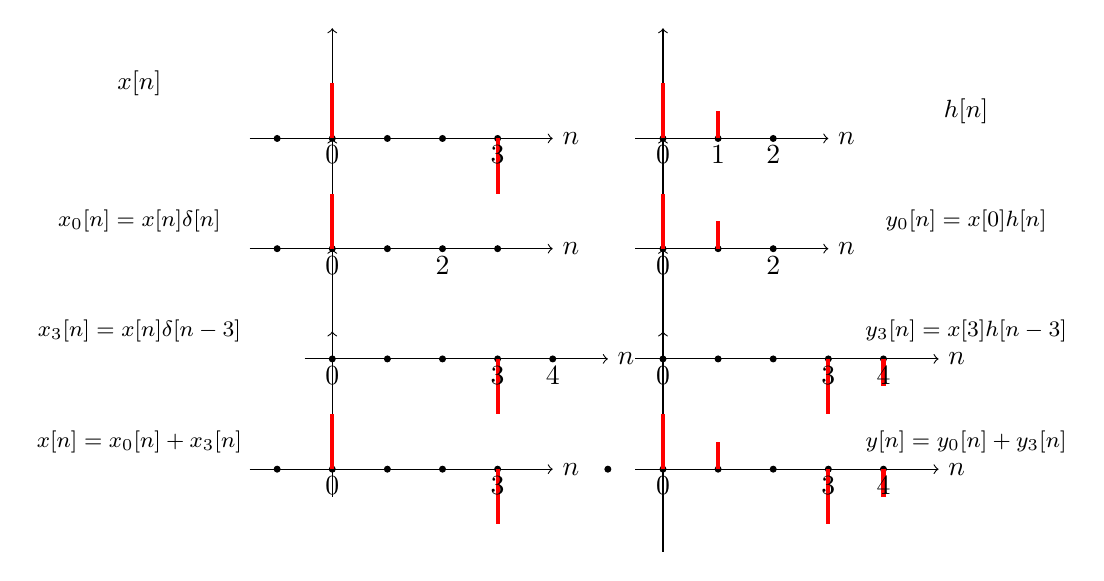
\begin{tikzpicture}[scale=0.7]
        % Top row: Input sequences
        % x[n]
        \begin{scope}[shift={(0,6)}]
            \draw[->] (-1.5,0) -- (4,0) node[right] {$n$};
            \draw[->] (0,-0.5) -- (0,2);
            \node[font=\small] at (-3.5,1) {$x[n]$};
            
            % Plot points
            \foreach \x in {-1,0,1,2,3} {
                \draw[fill] (\x,0) circle (1.5pt);
            }
            % Non-zero values (removed x[-2], keeping x[0] and x[3])
            \draw[thick, line width=1.5pt, red] (0,0) -- (0,1);
            \draw[thick, line width=1.5pt, red] (3,0) -- (3,-1);
            
            % Labels
            \node at (0,-0.3) {0};
            \node at (3,-0.3) {3};
        \end{scope}
        
        % h[n]
        \begin{scope}[shift={(6,6)}]
            \draw[->] (-0.5,0) -- (3,0) node[right] {$n$};
            \draw[->] (0,-0.5) -- (0,2);
            \node[font=\small] at (5.5,0.5) {$h[n]$};
            
            % Plot points
            \foreach \x in {0,1,2} {
                \draw[fill] (\x,0) circle (1.5pt);
            }
            % Non-zero values
            \draw[thick, line width=1.5pt, red] (0,0) -- (0,1);
            \draw[thick, line width=1.5pt, red] (1,0) -- (1,0.5);
            
            % Labels
            \node at (0,-0.3) {0};
            \node at (1,-0.3) {1};
            \node at (2,-0.3) {2};
        \end{scope}
        
        % Second row: x[0] components
        \begin{scope}[shift={(0,4)}]
            \draw[->] (-1.5,0) -- (4,0) node[right] {$n$};
            \draw[->] (0,-0.5) -- (0,2);
            \node[font=\footnotesize] at (-3.5,0.5) {$x_0[n] = x[n]\delta[n]$};
            
            \foreach \x in {-1,0,1,2,3} {
                \draw[fill] (\x,0) circle (1.5pt);
            }
            \draw[thick, line width=1.5pt, red] (0,0) -- (0,1);
            \node at (0,-0.3) {0};
            \node at (2,-0.3) {2};
        \end{scope}
        
        \begin{scope}[shift={(6,4)}]
            \draw[->] (-0.5,0) -- (3,0) node[right] {$n$};
            \draw[->] (0,-0.5) -- (0,2);
            \node[font=\footnotesize] at (5.5,0.5) {$y_0[n] = x[0]h[n]$};
            
            \foreach \x in {0,1,2} {
                \draw[fill] (\x,0) circle (1.5pt);
            }
            \draw[thick, line width=1.5pt, red] (0,0) -- (0,1);
            \draw[thick, line width=1.5pt, red] (1,0) -- (1,0.5);
            \node at (0,-0.3) {0};
            \node at (2,-0.3) {2};
        \end{scope}
        
        % Third row: x[3] components
        \begin{scope}[shift={(0,2)}]
            \draw[->] (-0.5,0) -- (5,0) node[right] {$n$};
            \draw[->] (0,-0.5) -- (0,2);
            \node[font=\footnotesize] at (-3.5,0.5) {$x_3[n] = x[n]\delta[n-3]$};
            
            \foreach \x in {0,1,2,3,4} {
                \draw[fill] (\x,0) circle (1.5pt);
            }
            \draw[thick, line width=1.5pt, red] (3,0) -- (3,-1);
            \node at (0,-0.3) {0};
            \node at (3,-0.3) {3};
            \node at (4,-0.3) {4};
        \end{scope}
        
        \begin{scope}[shift={(6,2)}]
            \draw[->] (-0.5,0) -- (5,0) node[right] {$n$};
            \draw[->] (0,-0.5) -- (0,2);
            \node[font=\footnotesize] at (5.5,0.5) {$y_3[n] = x[3]h[n-3]$};
            
            \foreach \x in {0,1,2,3,4} {
                \draw[fill] (\x,0) circle (1.5pt);
            }
            \draw[thick, line width=1.5pt, red] (3,0) -- (3,-1);
            \draw[thick, line width=1.5pt, red] (4,0) -- (4,-0.5);
            \node at (0,-0.3) {0};
            \node at (3,-0.3) {3};
            \node at (4,-0.3) {4};
        \end{scope}
        
        % Bottom row: Sum
        \begin{scope}[shift={(0,0)}]
            \draw[->] (-1.5,0) -- (4,0) node[right] {$n$};
            \draw[->] (0,-0.5) -- (0,2.5);
            \node[font=\footnotesize] at (-3.5,0.5) {$x[n] = x_0[n] + x_3[n]$};
            
            \foreach \x in {-1,0,1,2,3} {
                \draw[fill] (\x,0) circle (1.5pt);
            }
            \draw[thick, line width=1.5pt, red] (0,0) -- (0,1);
            \draw[thick, line width=1.5pt, red] (3,0) -- (3,-1);
            \node at (0,-0.3) {0};
            \node at (3,-0.3) {3};
        \end{scope}
        
        \begin{scope}[shift={(6,0)}]
            \draw[->] (-0.5,0) -- (5,0) node[right] {$n$};
            \draw[->] (0,-1.5) -- (0,2.5);
            \node[font=\footnotesize] at (5.5,0.5) {$y[n] = y_0[n] + y_3[n]$};
            
            \foreach \x in {-1,0,1,2,3,4} {
                \draw[fill] (\x,0) circle (1.5pt);
            }
            % Sum of components
            \draw[thick, line width=1.5pt, red] (0,0) -- (0,1);
            \draw[thick, line width=1.5pt, red] (1,0) -- (1,0.5);
            \draw[thick, line width=1.5pt, red] (3,0) -- (3,-1);
            \draw[thick, line width=1.5pt, red] (4,0) -- (4,-0.5);
            
            \node at (0,-0.3) {0};
            \node at (3,-0.3) {3};
            \node at (4,-0.3) {4};
        \end{scope}

    \end{tikzpicture}
\end{center}
\end{frame}



\begin{frame}{The Convolution Sum}
\begin{itemize}
    \item The equation:
    \[
        y[n] = \sum_{k=-\infty}^{\infty} x[k]h[n-k]
    \]
    is referred to as the \textbf{convolution sum}.
    \item We represent this by the operator notation:
    \[
        y[n] = x[n] * h[n]
    \]
    \item The operation of discrete-time convolution takes two sequences $x[n]$ and $h[n]$ and produces a third sequence $y[n]$.
\end{itemize}
\end{frame}


\begin{frame}{Transforming $h[k]$ into $h[n-k]$}
% \begin{itemize}
    % \item This slide demonstrates the transformation of $h[k]$ into $h[n-k]$ step by step:
    % \item
    \[
        y[n] = \sum_{k=-\infty}^{\infty} x[k]h[n-k]
    \]
    \begin{enumerate}
        \item The original sequence $h[k]$.
        \item Flipping around the y-axis to get $h[-k]$.
        \item Shifting by $n$ to get $h[n-k]$ (or equivalently $h[-(k-n)]$).
    \end{enumerate}
% \end{itemize}

\begin{center}
    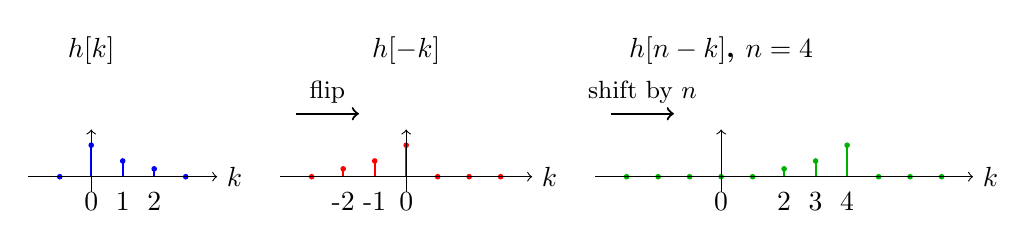
\begin{tikzpicture}[scale=0.4]
        % First plot: h[k]
        \begin{scope}[shift={(0,0)}]
            \node at (0, 4) {\textbf{$h[k]$}};
            
            % Plot h[k] - simple exponential decay starting at k=0
            \def\kmin{-1}
            \def\kmax{3}
            
            \foreach \k in {\kmin,...,\kmax} {
                \pgfmathsetmacro\hk{(\k == 0) * 1 + (\k == 1) * 0.5 + (\k == 2) * 0.25}
                \draw[thick, blue] (\k, 0) -- (\k, \hk);
                \filldraw[blue] (\k, \hk) circle (2pt);
            }
            
            % Axes
            \draw[->] (\kmin-1, 0) -- (\kmax+1, 0) node[right] {$k$};
            \draw[->] (0, -0.5) -- (0, 1.5);
            
            % Mark key points
            \node[below] at (0, -0.2) {0};
            \node[below] at (1, -0.2) {1};
            \node[below] at (2, -0.2) {2};
        \end{scope}
        
        % Second plot: h[-k] (flipped version)
        \begin{scope}[shift={(10,0)}]
            \node at (0, 4) {\textbf{$h[-k]$}};
            
            \def\kmin{-3}
            \def\kmax{3}
            
            \foreach \k in {\kmin,...,\kmax} {
                \pgfmathsetmacro\hk{(\k == 0) * 1 + (\k == -1) * 0.5 + (\k == -2) * 0.25}
                \draw[thick, red] (\k, 0) -- (\k, \hk);
                \filldraw[red] (\k, \hk) circle (2pt);
            }
            
            % Axes
            \draw[->] (\kmin-1, 0) -- (\kmax+1, 0) node[right] {$k$};
            \draw[->] (0, -0.5) -- (0, 1.5);
            
            % Mark key points
            \node[below] at (0, -0.2) {0};
            \node[below] at (-1, -0.2) {-1};
            \node[below] at (-2, -0.2) {-2};
        \end{scope}
        
        % Third plot: h[n-k] with n=4
        \begin{scope}[shift={(20,0)}]
            \node at (0, 4) {\textbf{$h[n-k]$, $n=4$}};
            
            \def\n{4} % Shift amount
            \def\kmin{-3}
            \def\kmax{7}
            
            \foreach \k in {\kmin,...,\kmax} {
                \pgfmathsetmacro\hk{(\k == \n) * 1 + (\k == \n-1) * 0.5 + (\k == \n-2) * 0.25}
                \draw[thick, green!70!black] (\k, 0) -- (\k, \hk);
                \filldraw[green!70!black] (\k, \hk) circle (2pt);
            }
            
            % Axes
            \draw[->] (\kmin-1, 0) -- (\kmax+1, 0) node[right] {$k$};
            \draw[->] (0, -0.5) -- (0, 1.5);
            
            % Mark key points
            \node[below] at (4, -0.2) {4};
            \node[below] at (3, -0.2) {3};
            \node[below] at (2, -0.2) {2};
            \node[below] at (0, -0.2) {0};
        \end{scope}
        
        % Add arrows between plots
        \draw[->, thick] (6.5, 2) -- (8.5, 2) node[midway, above] {\small flip};
        \draw[->, thick] (16.5, 2) -- (18.5, 2) node[midway, above] {\small shift by $n$};
        
    \end{tikzpicture}
\end{center}

\vspace{0.3cm}
\begin{itemize}
    \item Note: $h[n-k] = h[-(k-n)]$ represents $h[-k]$ shifted right by $n$ samples.
\end{itemize}
\end{frame}




\begin{frame}{Computing Convolution: Key Steps}
\begin{itemize}
    \item To compute $y[n]$, we need to form the sequence $h[n-k]$ for $-\infty < k < \infty$.
    \item Key insight: $h[n-k] = h[-(k-n)]$
    \item Steps to form $h[n-k]$ from $h[k]$:
    \begin{enumerate}
        \item Reverse $h[k]$ in time about $k = 0$ to get $h[-k]$
        \item Delay the time-reversed signal by $n$ samples to get $h[n-k]$
    \end{enumerate}
    \item Then multiply $x[k]$ and $h[n-k]$ sample by sample and sum all products.
\end{itemize}
\end{frame}


\begin{frame}{Example 1: Convolution of Two Sequences}
\begin{itemize}
    \item Consider a system with impulse response:
    \[
        h[n] = u[n] - u[n-N] = \begin{cases}
            1, & 0 \leq n \leq N-1 \\
            0, & \text{otherwise}
        \end{cases}
    \]
    \item Input signal:
    \[
        x[n] = a^n u[n] = \begin{cases}
            a^n, & n \geq 0 \\
            0, & n < 0
        \end{cases}
    \]
\end{itemize}
\end{frame}


% Case 1: n < 0
\begin{frame}{Example 1 : Convolution of Two Sequences (Case 1: $n < 0$)}
\begin{itemize}
    \item \textbf{Case 1:} $n < 0$
    \[
        y[n] = 0
    \]
    \item For $n < 0$, there is no overlap between $x[k]$ and $h[n-k]$, so the output is zero.
\end{itemize}

\begin{center}
    \begin{tikzpicture}[scale=0.4]
        % First subplot: x[k]
        \begin{scope}[shift={(0,6)}]
            % Plot x[k]
            \def\a{0.8} % Decay factor
            \def\kmin{-5} % Minimum value of k
            \def\kmax{15} % Maximum value of k
            
            \foreach \k in {\kmin,...,\kmax} {
                \pgfmathsetmacro\xk{(\k < 0) * 0 + (\k >= 0) * (\a^\k)}
                \draw[thick, blue] (\k, 0) -- (\k, \xk); % Stem line
                \filldraw[blue] (\k, \xk) circle (2pt); % Dot
            }
            
            % Axes
            \draw[->] (\kmin-1, 0) -- (\kmax+1, 0) node[right] {$k$}; % x-axis
            \draw[->] (0, -0.5) -- (0, 1.5) node[above] {$x[k] = a^k u[k]$};    % y-axis
        \end{scope}
        
        % Second subplot: h[n-k] (shifted out of range)
        \begin{scope}[shift={(0,0)}]
            % Plot h[n-k]
            \def\n{-3}  % Current value of n (example for n < 0)
            \def\N{5}   % Length of impulse response
            \def\kmin{-5} % Minimum value of k
            \def\kmax{15} % Maximum value of k
            
            \foreach \k in {\kmin,...,\kmax} {
                \pgfmathsetmacro\hnk{(\k > \n - \N && \k <= \n) * 1}
                \draw[thick, red] (\k, 0) -- (\k, \hnk); % Stem line
                \filldraw[red] (\k, \hnk) circle (2pt); % Dot
            }
            
            % Axes
            \draw[->] (\kmin-1, 0) -- (\kmax+1, 0) node[right] {$k$}; % x-axis
            \draw[->] (0, -0.5) -- (0, 1.5) node[above] {$h[n-k]$};   % y-axis
        \end{scope}
    \end{tikzpicture}
\end{center}

\end{frame}

% Case 2: 0 <= n <= N-1
\begin{frame}{Example 1 : Convolution of Two Sequences (Case 2: $0 \leq n \leq N-1$)}
\begin{itemize}
    \item \textbf{Case 2:} $0 \leq n \leq N-1$
    \[
        y[n] = \sum_{k=0}^{n} a^k = \frac{1-a^{n+1}}{1-a}
    \]
    \item For $0 \leq n \leq N-1$, there is partial overlap between $x[k]$ and $h[n-k]$.
\end{itemize}

\begin{center}
    \begin{tikzpicture}[scale=0.4]
        % First subplot: x[k]
        \begin{scope}[shift={(0,6)}]
            % Plot x[k]
            \def\a{0.8} % Decay factor
            \def\kmin{-5} % Minimum value of k
            \def\kmax{15} % Maximum value of k
            
            \foreach \k in {\kmin,...,\kmax} {
                \pgfmathsetmacro\xk{(\k < 0) * 0 + (\k >= 0) * (\a^\k)}
                \draw[thick, blue] (\k, 0) -- (\k, \xk); % Stem line
                \filldraw[blue] (\k, \xk) circle (2pt); % Dot
            }
            
            % Axes
            \draw[->] (\kmin-1, 0) -- (\kmax+1, 0) node[right] {$k$}; % x-axis
            \draw[->] (0, -0.5) -- (0, 1.5) node[above] {$x[k] = a^k u[k]$};    % y-axis
        \end{scope}
        
        % Second subplot: h[n-k] (partial overlap)
        \begin{scope}[shift={(0,0)}]
            % Plot h[n-k]
            \def\n{3}  % Current value of n (example for 0 <= n <= N-1)
            \def\N{5}   % Length of impulse response
            \def\kmin{-5} % Minimum value of k
            \def\kmax{15} % Maximum value of k
            
            \foreach \k in {\kmin,...,\kmax} {
                \pgfmathsetmacro\hnk{(\k > \n - \N && \k <= \n) * 1}
                \draw[thick, red] (\k, 0) -- (\k, \hnk); % Stem line
                \filldraw[red] (\k, \hnk) circle (2pt); % Dot
            }
            
            % Axes
            \draw[->] (\kmin-1, 0) -- (\kmax+1, 0) node[right] {$k$}; % x-axis
            \draw[->] (0, -0.5) -- (0, 1.5) node[above] {$h[n-k]$};   % y-axis
        \end{scope}
    \end{tikzpicture}
\end{center}

\end{frame}

% Case 3: n > N-1
\begin{frame}{Example 1 : Convolution of Two Sequences (Case 3: $n > N-1$)}
\begin{itemize}
    \item \textbf{Case 3:} $n > N-1$
    \[
        y[n] = \sum_{k=n-N+1}^{n} a^k = a^{n-N+1} \frac{1-a^N}{1-a}
    \]
    \item For $n > N-1$, there is full overlap between $x[k]$ and $h[n-k]$.
\end{itemize}

\begin{center}
    \begin{tikzpicture}[scale=0.4]
        % First subplot: x[k]
        \begin{scope}[shift={(0,6)}]
            % Plot x[k]
            \def\a{0.8} % Decay factor
            \def\kmin{-5} % Minimum value of k
            \def\kmax{15} % Maximum value of k
            
            \foreach \k in {\kmin,...,\kmax} {
                \pgfmathsetmacro\xk{(\k < 0) * 0 + (\k >= 0) * (\a^\k)}
                \draw[thick, blue] (\k, 0) -- (\k, \xk); % Stem line
                \filldraw[blue] (\k, \xk) circle (2pt); % Dot
            }
            
            % Axes
            \draw[->] (\kmin-1, 0) -- (\kmax+1, 0) node[right] {$k$}; % x-axis
            \draw[->] (0, -0.5) -- (0, 1.5) node[above] {$x[k] = a^k u[k]$};    % y-axis
        \end{scope}
        
        % Second subplot: h[n-k] (full overlap)
        \begin{scope}[shift={(0,0)}]
            % Plot h[n-k]
            \def\n{8}  % Current value of n (example for n > N-1)
            \def\N{5}   % Length of impulse response
            \def\kmin{-5} % Minimum value of k
            \def\kmax{15} % Maximum value of k
            
            \foreach \k in {\kmin,...,\kmax} {
                \pgfmathsetmacro\hnk{(\k > \n - \N && \k <= \n) * 1}
                \draw[thick, red] (\k, 0) -- (\k, \hnk); % Stem line
                \filldraw[red] (\k, \hnk) circle (2pt); % Dot
            }
            
            % Axes
            \draw[->] (\kmin-1, 0) -- (\kmax+1, 0) node[right] {$k$}; % x-axis
            \draw[->] (0, -0.5) -- (0, 1.5) node[above] {$h[n-k]$};   % y-axis
        \end{scope}
    \end{tikzpicture}
\end{center}

\end{frame}


\begin{frame}{Example 1: Complete Solution}
\begin{itemize}
    \item The complete closed-form expression for $y[n]$ is:
    \[
        y[n] = \begin{cases}
            0, & n < 0 \\
            \frac{1-a^{n+1}}{1-a}, & 0 \leq n \leq N-1 \\
            a^{n-N+1}\frac{1-a^N}{1-a}, & n > N-1
        \end{cases}
    \]
    \item Below is a visualization of $y[n]$ for $a = 0.8$ and $N = 5$.
\end{itemize}

\begin{center}
    \begin{tikzpicture}[scale=0.4]
        % Parameters
        \def\a{0.8} % Decay factor
        \def\N{5}   % Length of impulse response
        \def\nmin{-10} % Minimum value of n
        \def\nmax{20}  % Maximum value of n
        
        % Define the range of n
        \foreach \n in {\nmin,...,\nmax} {
            % Compute y[n] based on the cases
            \pgfmathsetmacro\yn{%
                (\n < 0) * 0 + 
                (0 <= \n && \n <= \N-1) * (1 - \a^(\n+1)) / (1 - \a) + 
                (\n > \N-1) * (\a^(\n-\N+1) * (1 - \a^\N) / (1 - \a))
            }
            
            % Plot the stem lines and dots
            \draw[thick, blue] (\n, 0) -- (\n, \yn); % Stem line
            \filldraw[blue] (\n, \yn) circle (2pt); % Dot
        }
        
        % Axes
        \draw[->] (\nmin-1, 0) -- (\nmax+1, 0) node[right] {$n$}; % x-axis
        \draw[->] (0, -1) -- (0, 6) node[above] {$y[n]$};        % y-axis

        % Labels
        \node at (1, -0.5) {$0$};
        \node at (\N-1, -0.5) {$N-1$};
        \node at (\N+2, -0.5) {$N$};
    \end{tikzpicture}
\end{center}
\end{frame}


\begin{frame}{Example 2: Convolution of Two Sequences}
\begin{itemize}
    \item Consider a system with impulse response:
    \[
        h[n] = u[n] - u[n-4] = \begin{cases}
            1, & 0 \leq n \leq 3 \\
            0, & \text{otherwise}
        \end{cases}
    \]
    \item Input signal:
    \[
        x[n] = u[n-2] - u[n-6] = \begin{cases}
            1, & 2 \leq n \leq 5 \\
            0, & \text{otherwise}
        \end{cases}
    \]
\end{itemize}
\end{frame}


\ifthenelse{\boolean{showresults}}{
\begin{frame}{Visualizing the Solution to Example 2}
\begin{center}
    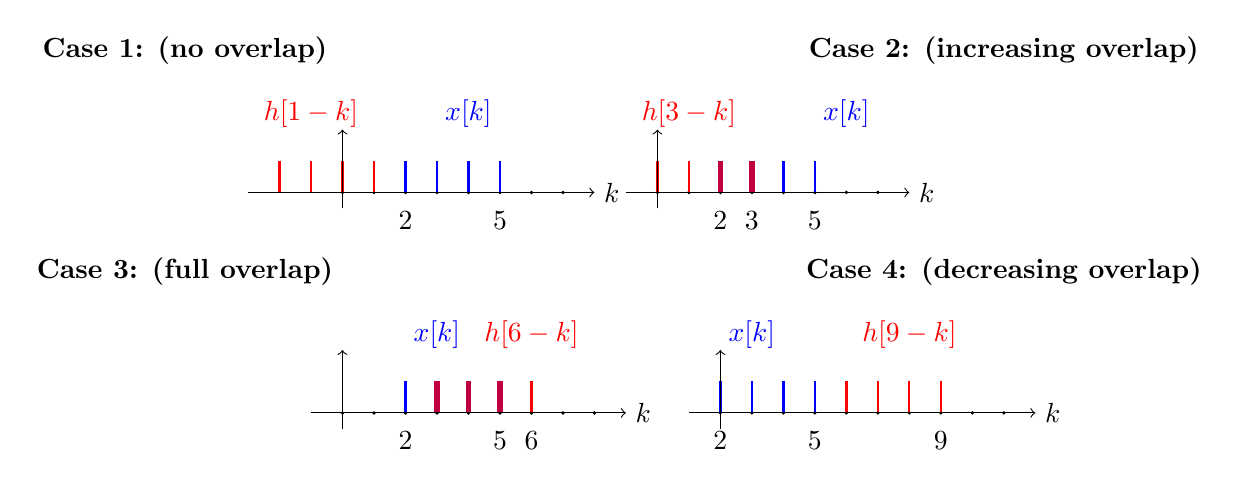
\begin{tikzpicture}[scale=0.4]
        % Case 1: n < 2 (n = 1 example)
        \begin{scope}[shift={(0,11)}]
            \node at (-5, 4.5) {\textbf{Case 1: (no overlap)}};
            % \node at (3, 4) {$y[1] = 0$};
            
            % Plot x[k] (blue)
            \foreach \k in {0,1,2,3,4,5,6,7} {
                \draw[fill] (\k, 0) circle (1pt);
                \pgfmathsetmacro\xk{(\k >= 2 && \k <= 5) ? 1 : 0}
                \draw[thick, blue] (\k, 0) -- (\k, \xk);
            }
            
            % Plot h[n-k] = h[1-k] (red, shifted left)
            \foreach \k in {-2,-1,0,1,2,3,4,5} {
                \pgfmathsetmacro\hnk{(\k >= -2 && \k <= 1) ? 1 : 0}
                \draw[thick, red] (\k, 0) -- (\k, \hnk);
            }
            
            % Axes and labels
            \draw[->] (-3, 0) -- (8, 0) node[right] {$k$};
            \draw[->] (0, -0.5) -- (0, 2);
            \node[below] at (2, -0.3) {2};
            \node[below] at (5, -0.3) {5};
            \node[blue] at (4, 2.5) {$x[k]$};
            \node[red] at (-1, 2.5) {$h[1-k]$};
        \end{scope}
        
        % Case 2: 2 ≤ n ≤ 5 (n = 3 example)
        \begin{scope}[shift={(10,11)}]
            \node at (11, 4.5) {\textbf{Case 2: (increasing overlap)}};
            % \node at (3, 4) {$y[3] = 2$};
            
            % Plot x[k] (blue)
            \foreach \k in {0,1,2,3,4,5,6,7} {
                \draw[fill] (\k, 0) circle (1pt);
                \pgfmathsetmacro\xk{(\k >= 2 && \k <= 5) ? 1 : 0}
                \draw[thick, blue] (\k, 0) -- (\k, \xk);
            }
            
            % Plot h[n-k] = h[3-k] (red)
            \foreach \k in {0,1,2,3,4,5,6} {
                \pgfmathsetmacro\hnk{(\k >= 0 && \k <= 3) ? 1 : 0}
                \draw[thick, red] (\k, 0) -- (\k, \hnk);
            }
            
            % Highlight overlap (purple)
            \foreach \k in {2,3} {
                \draw[thick, purple, line width=2pt] (\k, 0) -- (\k, 1);
            }
            
            % Axes and labels
            \draw[->] (-1, 0) -- (8, 0) node[right] {$k$};
            \draw[->] (0, -0.5) -- (0, 2);
            \node[below] at (2, -0.3) {2};
            \node[below] at (3, -0.3) {3};
            \node[below] at (5, -0.3) {5};
            \node[blue] at (6, 2.5) {$x[k]$};
            \node[red] at (1, 2.5) {$h[3-k]$};
        \end{scope}
        
        % Case 3: 6 ≤ n ≤ 8 (n = 6 example)
        \begin{scope}[shift={(0,4)}]
            \node at (-5, 4.5) {\textbf{Case 3: (full overlap)}};
            % \node at (3, 4) {$y[6] = 4$};
            
            % Plot x[k] (blue)
            \foreach \k in {0,1,2,3,4,5,6,7,8} {
                \draw[fill] (\k, 0) circle (1pt);
                \pgfmathsetmacro\xk{(\k >= 2 && \k <= 5) ? 1 : 0}
                \draw[thick, blue] (\k, 0) -- (\k, \xk);
            }
            
            % Plot h[n-k] = h[6-k] (red)
            \foreach \k in {2,3,4,5,6,7,8} {
                \pgfmathsetmacro\hnk{(\k >= 3 && \k <= 6) ? 1 : 0}
                \draw[thick, red] (\k, 0) -- (\k, \hnk);
            }
            
            % Highlight overlap (purple)
            \foreach \k in {3,4,5} {
                \draw[thick, purple, line width=2pt] (\k, 0) -- (\k, 1);
            }
            
            % Axes and labels
            \draw[->] (-1, 0) -- (9, 0) node[right] {$k$};
            \draw[->] (0, -0.5) -- (0, 2);
            \node[below] at (2, -0.3) {2};
            \node[below] at (5, -0.3) {5};
            \node[below] at (6, -0.3) {6};
            \node[blue] at (3, 2.5) {$x[k]$};
            \node[red] at (6, 2.5) {$h[6-k]$};
        \end{scope}
        
        % Case 4: n ≥ 9 (n = 9 example)
        \begin{scope}[shift={(10,4)}]
            \node at (11, 4.5) {\textbf{Case 4: (decreasing overlap)}};
            % \node at (3, 4) {$y[9] = 0$};
            
            % Plot x[k] (blue)
            \foreach \k in {2,3,4,5,6,7,8,9,10,11} {
                \draw[fill] (\k, 0) circle (1pt);
                \pgfmathsetmacro\xk{(\k >= 2 && \k <= 5) ? 1 : 0}
                \draw[thick, blue] (\k, 0) -- (\k, \xk);
            }
            
            % Plot h[n-k] = h[9-k] (red)
            \foreach \k in {5,6,7,8,9,10,11} {
                \pgfmathsetmacro\hnk{(\k >= 6 && \k <= 9) ? 1 : 0}
                \draw[thick, red] (\k, 0) -- (\k, \hnk);
            }
            
            % No overlap in this case
            
            % Axes and labels
            \draw[->] (1, 0) -- (12, 0) node[right] {$k$};
            \draw[->] (2, -0.5) -- (2, 2);
            \node[below] at (2, -0.3) {2};
            \node[below] at (5, -0.3) {5};
            \node[below] at (9, -0.3) {9};
            \node[blue] at (3, 2.5) {$x[k]$};
            \node[red] at (8, 2.5) {$h[9-k]$};
        \end{scope}

        
    \end{tikzpicture}
\end{center}
\end{frame}
}{}

\ifthenelse{\boolean{showresults}}{
\begin{frame}{Solution to Example 2}
    \begin{enumerate}
        \item \textbf{Case 1:} $n < 2$
        \[
            y[n] = 0 \quad \text{(no overlap between $x[k]$ and $h[n-k]$)}
        \]
        \item \textbf{Case 2:} $2 \leq n \leq 5$
        \[
            y[n] = \sum_{k=2}^{n} h[n-k] = \min(n-2+1, 4)
        \]
        \item \textbf{Case 3:} $6 \leq n \leq 8$
        \[
            y[n] = \sum_{k=n-3}^{5} h[n-k] = 4
        \]
        \item \textbf{Case 4:} $n \geq 9$
        \[
            y[n] = \sum_{k=n-3}^{5} h[n-k] = 6-n
        \]
    \end{enumerate}
\end{frame}
}{}

\ifthenelse{\boolean{showresults}}{
\begin{frame}{Complete Output for Example 2}
\begin{center}
    \begin{tikzpicture}[scale=0.6]
        % Output plot
        \begin{scope}[shift={(0,0)}]
            \node at (0, 7) {\textbf{Complete Output $y[n]$}};
            
            % Plot the complete output
            \foreach \n in {0,1,2,3,4,5,6,7,8,9,10} {
                \draw[fill] (\n, 0) circle (1pt);
                \pgfmathsetmacro\yn{0}
                \pgfmathparse{(\n==2) ? 1 : ((\n==3) ? 2 : ((\n==4) ? 3 : ((\n==5) ? 4 : ((\n==6) ? 4 : ((\n==7) ? 3 : ((\n==8) ? 2 : 0))))))}
                \pgfmathsetmacro\yn{\pgfmathresult}
                \draw[thick, green!70!black] (\n, 0) -- (\n, \yn);
            }
            
            % Axes and labels
            \draw[->] (-1, 0) -- (11, 0) node[right] {$n$};
            \draw[->] (0, -0.5) -- (0, 5);
            \node[below] at (2, -0.3) {2};
            \node[below] at (5, -0.3) {5};
            \node[below] at (8, -0.3) {8};
            \node[left] at (0, 4) {4};
        \end{scope}
        
    \end{tikzpicture}
\end{center}
\end{frame}
}{}

% \begin{frame}{Key Properties of Convolution}
% \begin{itemize}
%     \item \textbf{Computational Tool:} The convolution sum serves as an explicit realization of a discrete-time linear system.
%     \item \textbf{Complete Characterization:} Given sequences $x[n]$ and $h[n]$, we can compute each sample of $y[n]$.
%     \item \textbf{Practical Implementation:} The convolution sum can be implemented numerically for sampled data or analytically for sequences with known formulas.
%     \item Unlike continuous-time, the discrete convolution sum is not an approximation but an exact representation.
% \end{itemize}
% \end{frame}

% \begin{frame}{Summary}
% \begin{itemize}
%     \item LTI systems combine linearity and time invariance properties.
%     \item They are completely characterized by their impulse response $h[n]$.
%     \item The output is computed using the convolution sum:
%     \[
%         y[n] = \sum_{k=-\infty}^{\infty} x[k]h[n-k] = x[n] * h[n]
%     \]
%     \item Convolution provides both analytical insight and computational implementation for LTI systems.
%     \item The convolution operation is fundamental to discrete-time signal processing.
% \end{itemize}
% \end{frame}

\section{LTI System Properties}

\begin{frame}{Properties of Linear Time-Invariant (LTI) Systems}
\begin{itemize}
    \item LTI systems are defined by the convolution operation:
    \[
        y[n] = x[n] \ast h[n]
    \]
    \item The impulse response \( h[n] \) fully characterizes an LTI system.
    \item Key properties derive from the convolution operation:
    \begin{itemize}
        \item Commutativity
        \item Distributivity over addition
        \item Associativity
    \end{itemize}
\end{itemize}
\end{frame}

\begin{frame}{Commutativity of LTI Systems}
\begin{itemize}
    \item The convolution operation is commutative:
    \[
        x[n] \ast h[n] = h[n] \ast x[n]
    \]
    \item This means the order of the input signal and impulse response does not matter.
    \item Proof:
    \begin{align*}
        y[n] &= \sum_{k=-\infty}^\infty x[k] h[n-k] \\
             &= \sum_{m=-\infty}^\infty h[m] x[n-m] \quad \text{(substitute } m = n-k, \text{ so } k = n-m\text{)} \\
             &= h[n] \ast x[n]
    \end{align*}
    \item Implication:
    \begin{itemize}
        \item A system with input \( x[n] \) and impulse response \( h[n] \) produces the same output as a system with input \( h[n] \) and impulse response \( x[n] \).
    \end{itemize}
\end{itemize}
\end{frame}


\begin{frame}{Commutativity of LTI Systems: Cascade Connection}
\begin{center}
    \begin{tikzpicture}[scale=1, every node/.style={scale=0.9}, node distance=2cm, >=latex]
        % First group: h1 -> h2
        % Input x[n]
        \node (input) {\(x[n]\)};
        % First system h1[n]
        \node[draw, rectangle, minimum width=1.5cm, minimum height=1cm, right of=input, xshift=1.5cm] (h1) {\(h_1[n]\)};
        % Second system h2[n]
        \node[draw, rectangle, minimum width=1.5cm, minimum height=1cm, right of=h1, xshift=2cm] (h2) {\(h_2[n]\)};
        % Output y[n]
        \node[right of=h2, xshift=1.5cm] (output) {\(y[n]\)};
        % Arrows connecting blocks
        \draw[->] (input) -- (h1);
        \draw[->] (h1) -- node[above] {} (h2);
        \draw[->] (h2) -- (output);

        % Second group: h2 -> h1
        % Input x[n]
        \node[below of=input, yshift=-1cm] (input_swapped) {\(x[n]\)};
        % First system h2[n]
        \node[draw, rectangle, minimum width=1.5cm, minimum height=1cm, right of=input_swapped, xshift=1.5cm] (h2_swapped) {\(h_2[n]\)};
        % Second system h1[n]
        \node[draw, rectangle, minimum width=1.5cm, minimum height=1cm, right of=h2_swapped, xshift=2cm] (h1_swapped) {\(h_1[n]\)};
        % Output y[n]
        \node[right of=h1_swapped, xshift=1.5cm] (output_swapped) {\(y[n]\)};
        % Arrows connecting swapped blocks
        \draw[->] (input_swapped) -- (h2_swapped);
        \draw[->] (h2_swapped) -- node[above] {} (h1_swapped);
        \draw[->] (h1_swapped) -- (output_swapped);

        % Third group: Combined system h[n] = h1[n] * h2[n]
        % Input x[n]
        \node[below of=input_swapped, yshift=-1cm] (input_combined) {\(x[n]\)};
        % Combined system h[n]
        \node[draw, rectangle, minimum width=2.5cm, minimum height=1cm, right of=input_combined, xshift=3cm] (combined) {\(h[n] = h_1[n] \ast h_2[n]\)};
        % Output y[n]
        \node[right of=combined, xshift=3cm] (output_combined) {\(y[n]\)};
        % Arrows connecting combined system
        \draw[->] (input_combined) -- (combined);
        \draw[->] (combined) -- (output_combined);
    \end{tikzpicture}
\end{center}
\end{frame}




\begin{frame}{Distributivity of LTI Systems}
\begin{itemize}
    \item The convolution operation distributes over addition:
    \[
        x[n] \ast (h_1[n] + h_2[n]) = x[n] \ast h_1[n] + x[n] \ast h_2[n]
    \]
    \item This property allows parallel systems to be simplified into a single equivalent system.
    \item Example (Parallel Combination):
    \begin{itemize}
        \item Two systems with impulse responses \( h_1[n] \) and \( h_2[n] \).
        \item Equivalent system impulse response:
        \[
            h[n] = h_1[n] + h_2[n]
        \]
    \end{itemize}
\end{itemize}
\end{frame}

\begin{frame}{Block Diagram: Distributivity of LTI Systems}
\begin{center}
    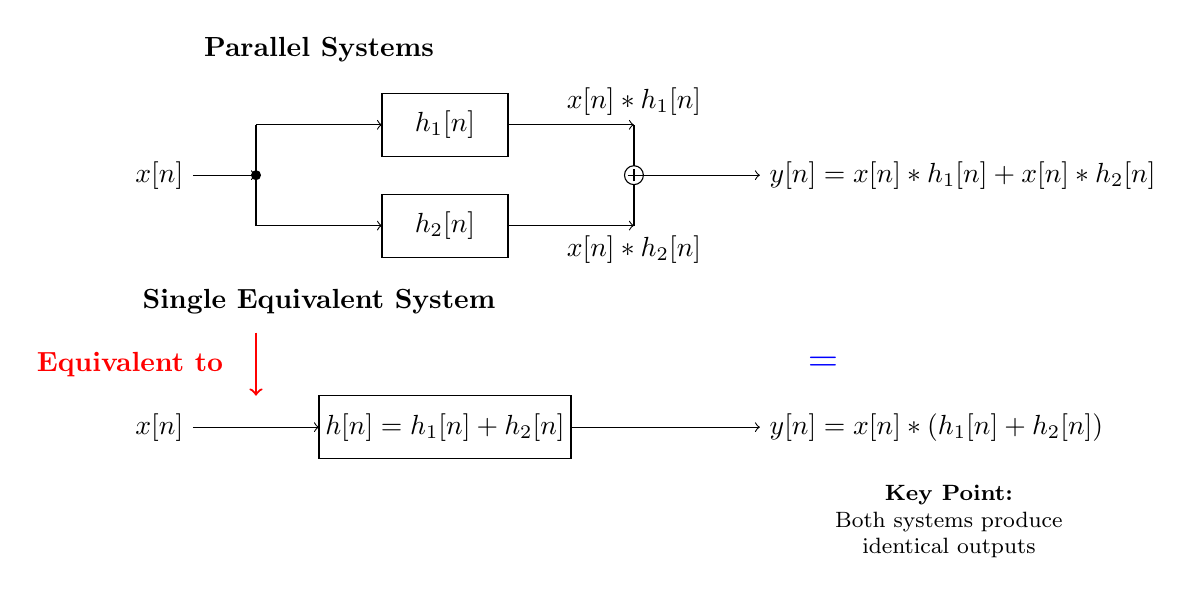
\begin{tikzpicture}[scale=0.8]
        % Top diagram: Parallel systems
        \begin{scope}[shift={(0,4)}]
            \node at (0, 2) {\textbf{Parallel Systems}};
            
            % Input
            \draw[->] (-2, 0) -- (-1, 0);
            \node[left] at (-2, 0) {$x[n]$};
            
            % Split point
            \filldraw (-1, 0) circle (2pt);
            \draw (-1, 0) -- (-1, 0.8);
            \draw (-1, 0) -- (-1, -0.8);
            
            % Upper branch - h1[n]
            \draw[->] (-1, 0.8) -- (1, 0.8);
            \draw (1, 0.3) rectangle (3, 1.3);
            \node at (2, 0.8) {$h_1[n]$};
            \draw[->] (3, 0.8) -- (5, 0.8);
            
            % Lower branch - h2[n]
            \draw[->] (-1, -0.8) -- (1, -0.8);
            \draw (1, -1.3) rectangle (3, -0.3);
            \node at (2, -0.8) {$h_2[n]$};
            \draw[->] (3, -0.8) -- (5, -0.8);
            
            % Summer - circle with plus
            \draw (5, -0.8) -- (5, -0.15);
            \draw (5, 0.8) -- (5, 0.15);
            \draw (5, 0) circle (0.15);
            \draw (4.9, 0) -- (5.1, 0);
            \draw (5, -0.1) -- (5, 0.1);
            
            % Output
            \draw[->] (5, 0) -- (7, 0);
            \node[right] at (7, 0) {$y[n] = x[n] \ast h_1[n] + x[n] \ast h_2[n]$};
            
            % Labels for branches
            \node[above] at (5, 0.8) {$x[n] \ast h_1[n]$};
            \node[below] at (5, -0.8) {$x[n] \ast h_2[n]$};
        \end{scope}
        
        % Equivalence arrow
        \draw[->, thick, red] (-1, 1.5) -- (-1, 0.5);
        \node[red] at (-3, 1) {\textbf{Equivalent to}};
        
        % Bottom diagram: Single equivalent system
        \begin{scope}[shift={(0,0)}]
            \node at (0, 2) {\textbf{Single Equivalent System}};
            
            % Input
            \draw[->] (-2, 0) -- (0, 0);
            \node[left] at (-2, 0) {$x[n]$};
            
            % Single system block
            \draw (0, -0.5) rectangle (4, 0.5);
            \node at (2, 0) {$h[n] = h_1[n] + h_2[n]$};
            
            % Output
            \draw[->] (4, 0) -- (7, 0);
            \node[right] at (7, 0) {$y[n] = x[n] \ast (h_1[n] + h_2[n])$};
        \end{scope}
        
        % Mathematical equivalence
        \node[blue, font=\Large] at (8, 1) {$=$};
        
        % Side note
        \node[align=center, font=\footnotesize] at (10, -1.5) {
            \textbf{Key Point:}\\
            Both systems produce\\
            identical outputs
        };
        
    \end{tikzpicture}
\end{center}
\end{frame}



% \begin{frame}{Associativity of Convolution}
% \begin{itemize}
%     \item Convolution is associative:
%     \[
%         (x[n] \ast h_1[n]) \ast h_2[n] = x[n] \ast (h_1[n] \ast h_2[n])
%     \]
%     \item Implication:
%     \begin{itemize}
%         \item Cascaded systems can be simplified:
%         \[
%             h[n] = h_1[n] \ast h_2[n]
%         \]
%     \end{itemize}
%     \item Example:
%     \[
%         y[n] = (x[n] \ast h_1[n]) \ast h_2[n] = x[n] \ast (h_1[n] \ast h_2[n])
%     \]
% \end{itemize}
% \end{frame}



\begin{frame}{Stability and Causality of LTI Systems}
\begin{itemize}
    \item Stability:
    \begin{itemize}
        \item An LTI system is stable if its impulse response is absolutely summable:
        \[
            \sum_{n=-\infty}^\infty |h[n]| < \infty
        \]
    \end{itemize}
    \item Causality:
    \begin{itemize}
        \item An LTI system is causal if \( h[n] = 0 \) for \( n < 0 \).
    \end{itemize}
    \item Example:
    \begin{itemize}
        \item The accumulator with \( h[n] = u[n] \) is causal but not stable.
        \item A system with \( h[n] = a^n u[n] \), \( |a| < 1 \), is both causal and stable.
    \end{itemize}
\end{itemize}
\end{frame}

\begin{frame}{Simplifications Using Convolution Properties}
\begin{itemize}
    \item Delay System:
    \[
        x[n] \ast \delta[n - n_d] = x[n - n_d]
    \]
    \item Example: Cascading Systems
    \begin{itemize}
        \item Forward Difference:
        \[
            h_1[n] = \delta[n+1] - \delta[n]
        \]
        \item Delay:
        \[
            h_2[n] = \delta[n-1]
        \]
        \item Equivalent system:
        \[
            h[n] = h_1[n] \ast h_2[n] = \delta[n] - \delta[n-1]
        \]
    \end{itemize}
\end{itemize}
\end{frame}






% ------------------------------------------------------------------------------------

\section{Stability of LTI Systems}


% \begin{frame}{Why Study Causality and Stability in LTI Systems?}
% \begin{itemize}
%     \item \textbf{LTI Systems have Special Properties}:
%     \begin{itemize}
%         \item Linearity and time invariance define a very special class of systems
%         \item These constraints make analysis much more tractable
%         \item We can determine system properties directly from the impulse response
%     \end{itemize}
    
%     \item \textbf{Easier Analysis for LTI Systems}:
%     \begin{itemize}
%         \item \textbf{Stability}: Check if $\sum_{n=-\infty}^\infty |h[n]| < \infty$
%         \item \textbf{Causality}: Check if $h[n] = 0$ for $n < 0$
%         \item No need to test with multiple inputs - impulse response tells us everything!
%     \end{itemize}

%     \item \textbf{Practical Importance}:
%     \begin{itemize}
%         \item Stability ensures bounded outputs for bounded inputs
%         \item Causality determines if system is physically realizable
%         \item Critical for system design and implementation
%     \end{itemize}
% \end{itemize}
% \end{frame}

\begin{frame}{Stability of LTI Systems}
    \begin{itemize}
        \item \textbf{Definition}: A stable system produces bounded output for every bounded input (BIBO)
        
        \item \textbf{LTI Stability Condition}:
        \[
            \text{System is stable} \iff \sum_{n=-\infty}^\infty |h[n]| < \infty
        \]
        
        \item \textbf{Proof}:
        \begin{itemize}
            \item \textit{Sufficient}: If $\sum |h[n]| < \infty$ and $|x[n]| \leq B_x$, then:
            \[
                |y[n]| = \left|\sum_{k=-\infty}^\infty h[k]x[n-k]\right| \leq \sum_{k=-\infty}^\infty |h[k]||x[n-k]| \leq B_x \sum_{k=-\infty}^\infty |h[k]|
            \]
            
            \item \textit{Necessary}: If $\sum |h[n]| = \infty$, we can construct a bounded input that produces unbounded output
        \end{itemize}
        
        \item \textbf{Key Insight}: For LTI systems, stability depends only on the impulse response!
    \end{itemize}
\end{frame}

\begin{frame}{Causality of LTI Systems}
    \begin{itemize}
        \item \textbf{Definition}: A causal system's output at time $n_0$ depends only on inputs at times $n \leq n_0$
        
        \item \textbf{LTI Causality Condition}:
        \[
            \text{System is causal} \iff h[n] = 0 \text{ for } n < 0
        \]
        
        \item \textbf{Justification}:
        \begin{itemize}
            \item From convolution: $y[n] = \sum_{k=-\infty}^\infty h[k]x[n-k]$
            \item For causality: $y[n]$ should not depend on $x[m]$ for $m > n$
            \item This requires $h[k] = 0$ when $n-k > n$, i.e., when $k < 0$
        \end{itemize}
        
        \item \textbf{Terminology}:
        \begin{itemize}
            \item A sequence that is zero for $n < 0$ is called a \textit{causal sequence}
            \item Such sequences could be impulse responses of causal systems
        \end{itemize}
    \end{itemize}
\end{frame}



\begin{frame}{Example 1: Ideal Delay System}
    \textbf{Problem}: Analyze the stability and causality of the ideal delay system.

    \vspace{0.3cm}
    \textbf{System Definition}:
    \[
        y[n] = x[n - n_d]
    \]
    where $n_d$ is a fixed integer (positive, negative, or zero).

    \vspace{0.3cm}
    \textbf{Find}:
    \begin{enumerate}
        \item The impulse response $h[n]$
        \item Determine if the system is stable
        \item Determine if the system is causal
    \end{enumerate}
\end{frame}

\ifthenelse{\boolean{showresults}}{
\begin{frame}{Example 1: Ideal Delay System - Solution}
    \textbf{Solution}:

    \vspace{0.2cm}
    \textbf{1. Impulse Response}:
    \[
        h[n] = \delta[n - n_d]
    \]

    \vspace{0.2cm}
    \textbf{2. Stability Analysis}:
    \[
        \sum_{n=-\infty}^\infty |h[n]| = \sum_{n=-\infty}^\infty |\delta[n - n_d]| = 1 < \infty
    \]
    $\Rightarrow$ \textcolor{green}{\textbf{System is STABLE}}

    \vspace{0.2cm}
    \textbf{3. Causality Analysis}:
    \begin{itemize}
        \item If $n_d \geq 0$: $h[n] = 0$ for $n < 0$ $\Rightarrow$ \textcolor{green}{\textbf{CAUSAL}}
        \item If $n_d < 0$: $h[n_d] = 1$ with $n_d < 0$ $\Rightarrow$ \textcolor{red}{\textbf{NON-CAUSAL}}
    \end{itemize}

    \vspace{0.2cm}
    \textbf{Conclusion}: All delay systems are stable. Causality depends on the sign of the delay.
\end{frame}
}{}


\begin{frame}{Example 2: Moving Average System}
    \textbf{Problem}: Analyze the stability and causality of the moving average system.

    \vspace{0.3cm}
    \textbf{System Definition}:
    \[
        y[n] = \frac{1}{M_1 + M_2 + 1} \sum_{k=-M_1}^{M_2} x[n-k]
    \]
    where $M_1$ and $M_2$ are non-negative integers.

    \vspace{0.3cm}
    \textbf{Find}:
    \begin{enumerate}
        \item The impulse response $h[n]$
        \item Determine if the system is stable
        \item Determine conditions for causality
    \end{enumerate}
\end{frame}

\ifthenelse{\boolean{showresults}}{
\begin{frame}{Example 2: Moving Average System - Solution}
    % \textbf{Solution}:

    % \vspace{0.2cm}
    \textbf{1. Impulse Response}:
    \[
        h[n] = \begin{cases}
            \frac{1}{M_1 + M_2 + 1}, & -M_1 \leq n \leq M_2 \\
            0, & \text{otherwise}
        \end{cases}
    \]

    % \vspace{0.2cm}
    \textbf{2. Stability Analysis}:
    \[
        \sum_{n=-\infty}^\infty |h[n]| = \sum_{n=-M_1}^{M_2} \frac{1}{M_1 + M_2 + 1} = \frac{M_1 + M_2 + 1}{M_1 + M_2 + 1} = 1 < \infty
    \]
    $\Rightarrow$ \textcolor{green}{\textbf{System is STABLE}} (FIR system with finite values)

    % \vspace{0.2cm}
    \textbf{3. Causality Analysis}:
    \begin{itemize}
        \item For causality: $h[n] = 0$ for $n < 0$
        \item This requires $-M_1 \geq 0$, so $M_1 = 0$
        \item \textbf{Causal moving average}: $M_1 = 0$, $M_2 \geq 0$
    \end{itemize}
\end{frame}
}{}

\begin{frame}{Example 3: Accumulator System}
    \textbf{Problem}: Analyze the stability and causality of the accumulator system.

    \vspace{0.3cm}
    \textbf{System Definition}:
    \[
        y[n] = \sum_{k=-\infty}^n x[k]
    \]

    \vspace{0.3cm}
    \textbf{Find}:
    \begin{enumerate}
        \item The impulse response $h[n]$
        \item Determine if the system is stable
        \item Determine if the system is causal
    \end{enumerate}
\end{frame}

\ifthenelse{\boolean{showresults}}{
\begin{frame}{Example 3: Accumulator System - Solution}
    \textbf{Solution}:

    \vspace{0.2cm}
    \textbf{1. Impulse Response}:
    \[
        h[n] = \sum_{k=-\infty}^n \delta[k] = u[n] = \begin{cases}
            1, & n \geq 0 \\
            0, & n < 0
        \end{cases}
    \]

    \vspace{0.2cm}
    \textbf{2. Stability Analysis}:
    \[
        \sum_{n=-\infty}^\infty |h[n]| = \sum_{n=0}^\infty |u[n]| = \sum_{n=0}^\infty 1 = \infty
    \]
    $\Rightarrow$ \textcolor{red}{\textbf{System is UNSTABLE}}

    \vspace{0.2cm}
    \textbf{3. Causality Analysis}:
    \[
        h[n] = 0 \text{ for } n < 0
    \]
    $\Rightarrow$ \textcolor{green}{\textbf{System is CAUSAL}}

    \vspace{0.2cm}
    \textbf{Conclusion}: The accumulator is causal but unstable (IIR system).
\end{frame}
}{}

\begin{frame}{Example 4: Exponential System}
    \textbf{Problem}: Analyze the stability and causality of the exponential system.

    \vspace{0.3cm}
    \textbf{System Definition}:
    \[
        h[n] = a^n u[n]
    \]
    where $a$ is a real constant.

    \vspace{0.3cm}
    \textbf{Find}:
    \begin{enumerate}
        \item Determine conditions for stability
        \item Determine if the system is causal
        \item What happens for different values of $|a|$?
    \end{enumerate}
\end{frame}

\ifthenelse{\boolean{showresults}}{
\begin{frame}{Example 4: Exponential System - Solution}
    \textbf{Solution}:

    \vspace{0.2cm}
    \textbf{1. Stability Analysis}:
    \[
        \sum_{n=-\infty}^\infty |h[n]| = \sum_{n=0}^\infty |a|^n
    \]

    \begin{itemize}
        \item If $|a| < 1$: $\sum_{n=0}^\infty |a|^n = \frac{1}{1-|a|} < \infty$ $\Rightarrow$ \textcolor{green}{\textbf{STABLE}}
        \item If $|a| \geq 1$: $\sum_{n=0}^\infty |a|^n = \infty$ $\Rightarrow$ \textcolor{red}{\textbf{UNSTABLE}}
    \end{itemize}

    \vspace{0.2cm}
    \textbf{2. Causality Analysis}:
    \[
        h[n] = a^n u[n] = 0 \text{ for } n < 0
    \]
    $\Rightarrow$ \textcolor{green}{\textbf{System is CAUSAL}}

    \vspace{0.2cm}
    \textbf{Conclusion}: The system is always causal. Stability depends on $|a| < 1$.
\end{frame}
}{}

\begin{frame}{Summary: Stability and Causality Examples}
    \begin{center}
    \begin{tabular}{|l|c|c|c|}
    \hline
    \textbf{System} & \textbf{Impulse Response} & \textbf{Stable?} & \textbf{Causal?} \\
    \hline
    Ideal Delay & $\delta[n-n_d]$ & \textcolor{green}{Yes} & \textcolor{green}{Yes} if $n_d \geq 0$ \\
    & & & \textcolor{red}{No} if $n_d < 0$ \\
    \hline
    Moving Average & $\frac{1}{M_1+M_2+1}$ & \textcolor{green}{Yes} & \textcolor{green}{Yes} if $M_1 = 0$ \\
    & & & \textcolor{red}{No} if $M_1 > 0$ \\
    \hline
    Accumulator & $u[n]$ & \textcolor{red}{No} & \textcolor{green}{Yes} \\
    \hline
    Exponential & $a^n u[n]$ & \textcolor{green}{Yes} if $|a|<1$ & \textcolor{green}{Yes} \\
    & & \textcolor{red}{No} if $|a| \geq 1$ & \\
    % \hline
    % Forward Difference & $\delta[n+1]-\delta[n]$ & \textcolor{green}{Yes} & \textcolor{red}{No} \\
    % \hline
    % Backward Difference & $\delta[n]-\delta[n-1]$ & \textcolor{green}{Yes} & \textcolor{green}{Yes} \\
    \hline
    \end{tabular}
    \end{center}

    \vspace{0.3cm}
    \textbf{Key Observations}:
    \begin{itemize}
        \item FIR systems (finite impulse response) are always stable
        \item IIR systems (infinite impulse response) may or may not be stable
        \item Causality is determined by whether $h[n] = 0$ for $n < 0$
    \end{itemize}
\end{frame}


\end{document}
